\documentclass{article}
\usepackage{graphicx}
\usepackage[margin=cm]{geometry}

\begin{document}
    
    \title{\textbf{ICS Problem set 10}}
    \maketitle

    \section{1}
    \begin{center}
        \begin{tabular}{ | c | c | c | c | }
            \hline
            s & Machine Code & Assembly Code & Description \\
            \hline
            0 & 001 1 0001 & LOAD \#1 & Load the value 1 into the accumulator \\
            \hline
            1 & 010 0 1111 & STORE 15 & Store the value in the accumulator to memory address 15 \\
            \hline
            2 & 001 1 0000 & LOAD \#0 & Load the value 0 into the accumulator \\
            \hline
            3 & 101 1 0100 & EQUAL \#4 & If value in the accumulator equals to 4 skip the next step \\
            \hline
            4 & 110 1 0110 & JUMP \#6 & Jump to operation number 6 \\
            \hline
            5 & 111 1 0000 & HALT & Stop Execution \\
            \hline
            6 & 001 0 0011 & LOAD 3 & Load the value in memory address 3 to the accumulator \\
            \hline
            7 & 100 1 0001 & SUB \#1 & Subtract 1 from the accumulator \\
            \hline
            8 & 010 0 0011 & STORE 3 & Store the value in the accumulator to memory address 3 \\
            \hline
            9 & 001 0 1111 & LOAD 15 & Load the value in memory address 15 to the accumulator \\
            \hline
            10 & 011 0 1111 & ADD 15 & Add the value in memory address 15 to the accumulator \\
            \hline
            11 & 010 0 1111 & STORE 15 & Store the value in the accumulator to memory address 15 \\
            \hline
            12 & 110 1 0010 & JUMP 2 & Jump to operation defined in memory address 2 \\
            \hline
            13 & 000 0 0000 & Memory & Memory Address 13 \\
            \hline
            14 & 000 0 0000 & Memory & Memory Address 14 \\
            \hline
            15 & 000 0 0000 & Memory & Memory Address 15 \\
            \hline
        \end{tabular}
    \end{center}
    First 1 is loaded into the accumulator(0) and then stored in memory address 15(1). Then 0 is loaded into the accumulator(2) and then checked if it is equal to 4(3).
    Since the evaluation is false, the next step is not skipped. The value used by the equal statement is decreased by 1(6 and 7).
    Then the program adds the value stored into memory 15 to itself (9, 10, and 11). The program jumps back to instruction at memory address 2. Eventually, number used by the
    equal statement is 0. When this happens, execution is stopped(5).\\
	\\
    This specific program is computing the following expression:\\
    \\
    (2(2(2(2(a)))))\\
    \\
    where a = 1.\\
    \\
    \pagebreak
    
    \section{2}
    The timing diagram is: Figure 1\\
    \\
    \begin{figure}
        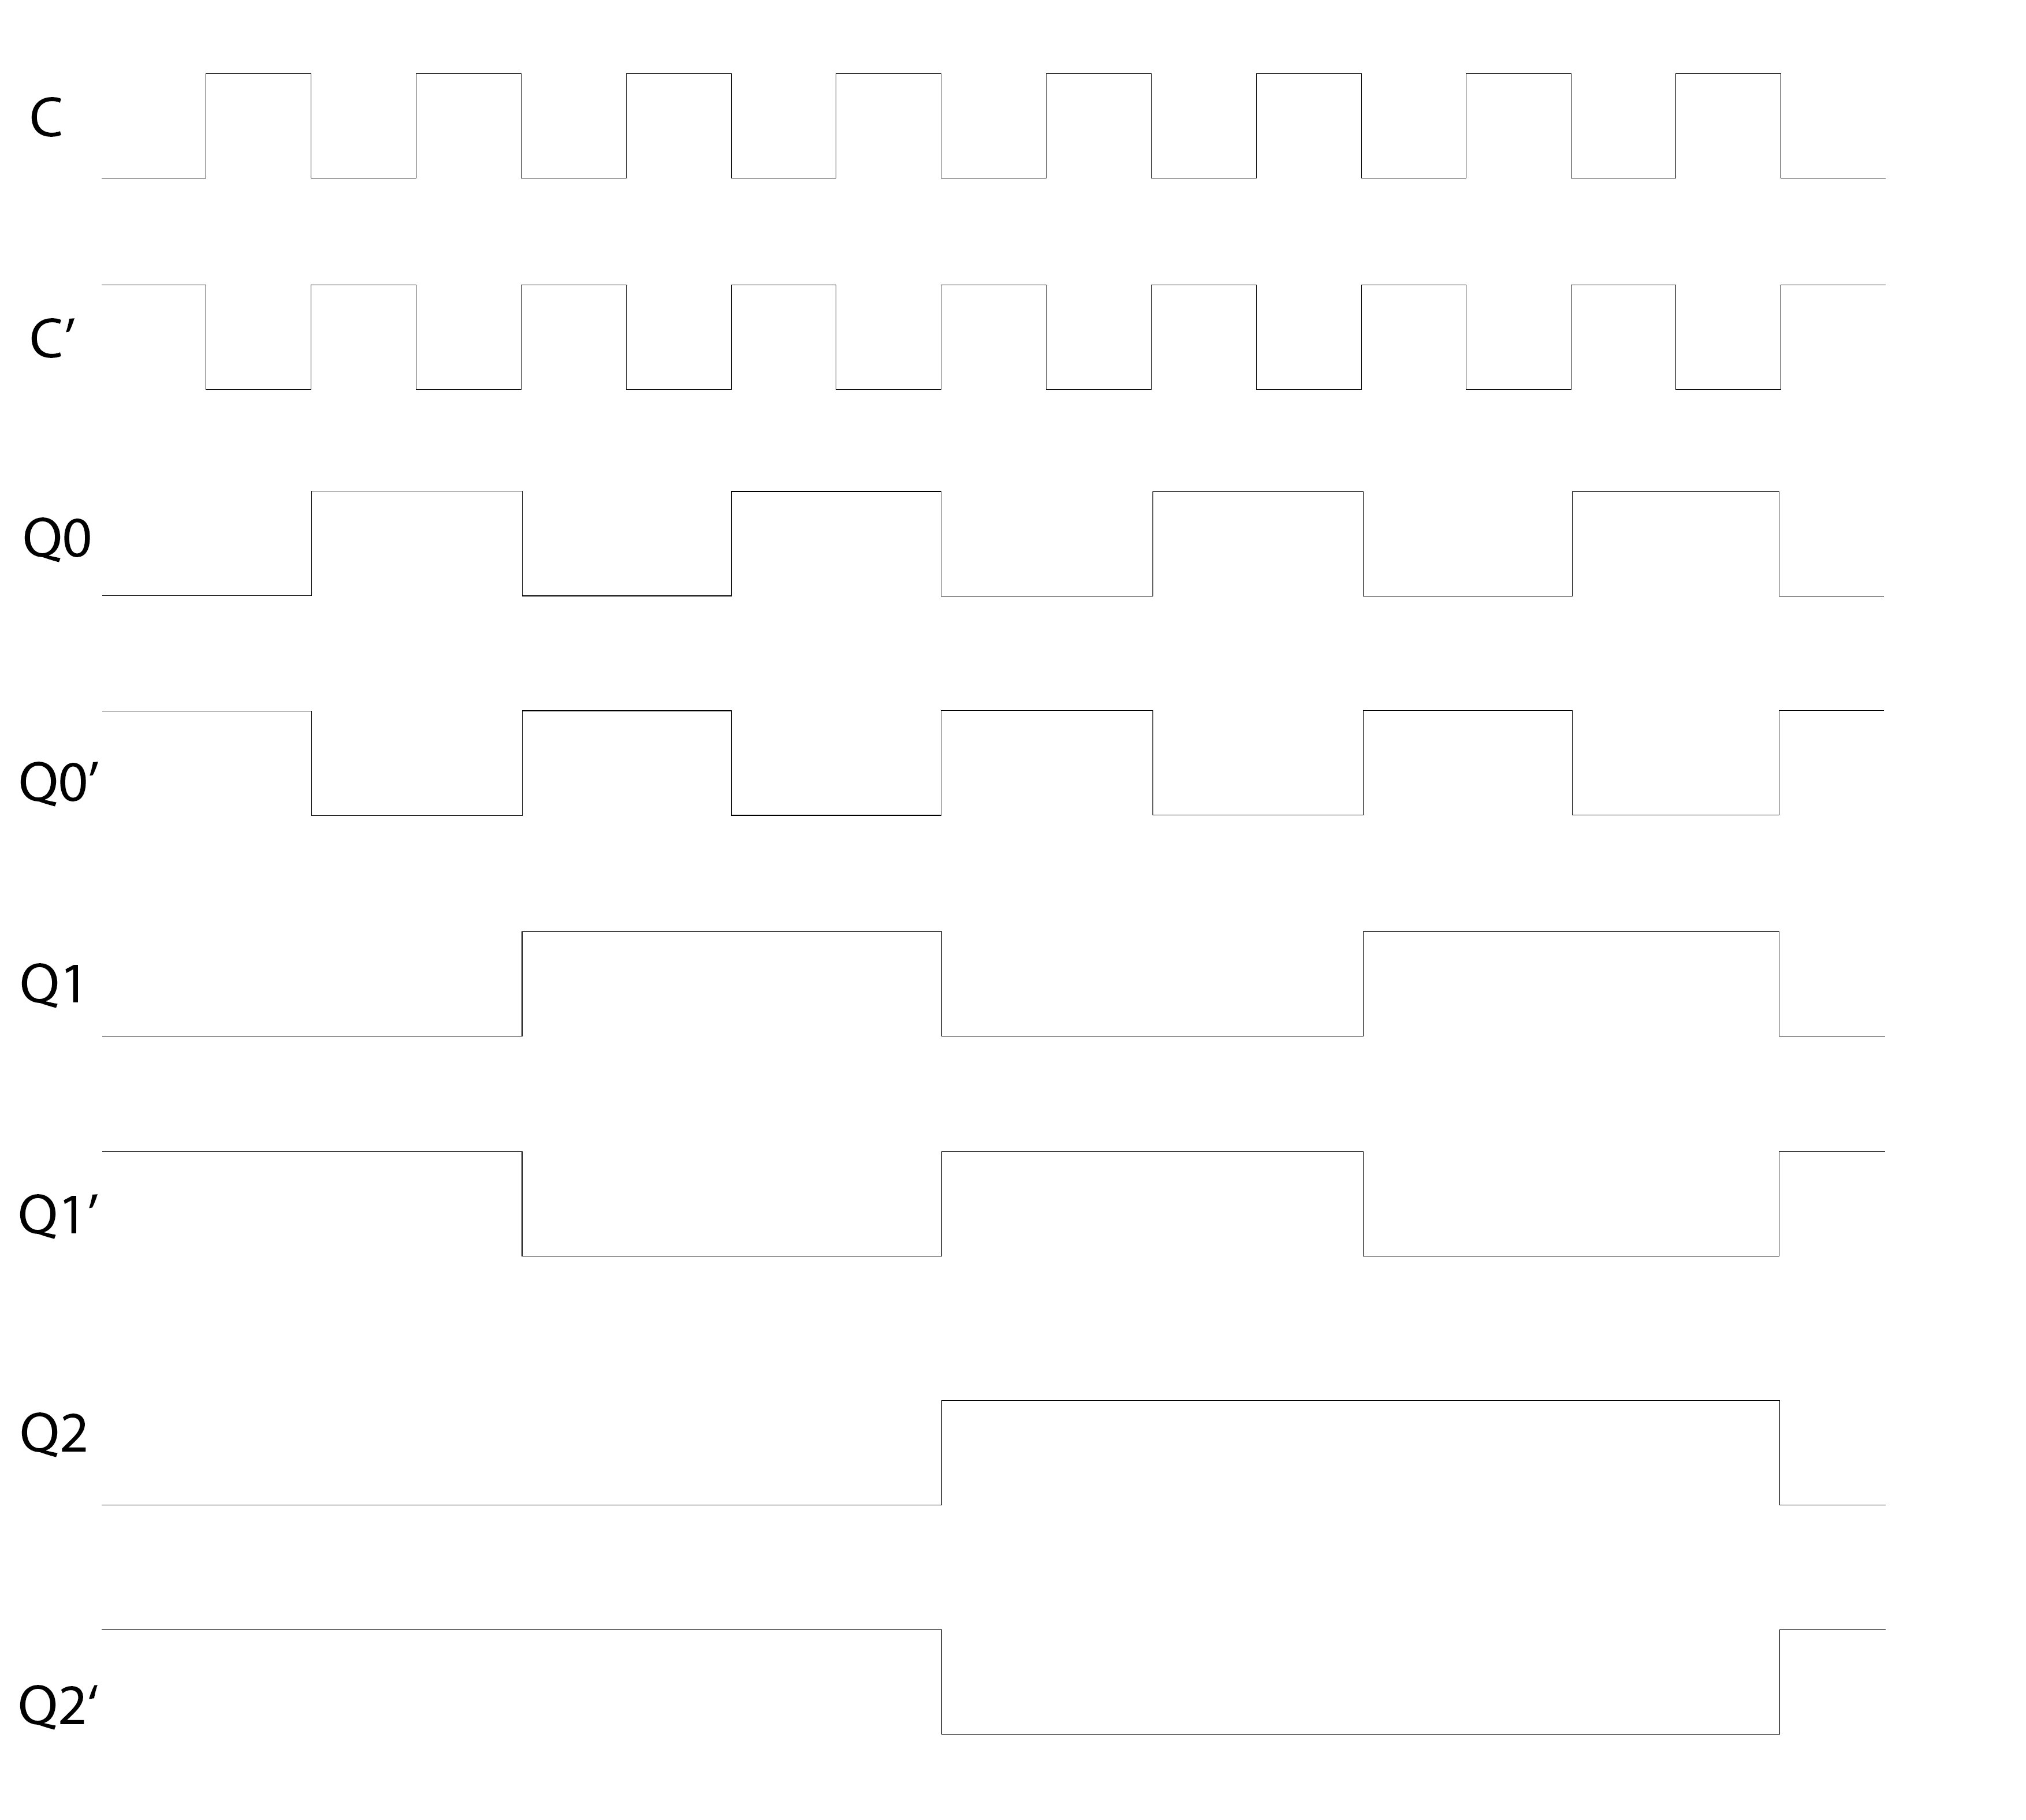
\includegraphics[height=12cm, angle=0]{FlipFlop.png}
        \caption{Signal diagram with no gate delays}
    \end{figure}
    Theoretically you could make your flip flop arbitrary long if you do not consider the gate delay. However, realistically, the gate delay will
    lead to the output signal being delayed in reference to the clock signal.
    \pagebreak

\end{document}